
\chapter{Kreslenie molekuly}

Po tom co ziskame a aplikujeme mapovanie medzi sablonovou a cielovou molekulou RNA,
ziskame cielovu molekulu s ciastocnou vizualizaciou, ktorej zvysok treba dopocitat.

Po operaciach delete ostavaju v molekule prazdne diery, naopak po insertoch potrebujeme
vypocitat, kam umiestnime bazovy par, resp. samotnu bazu, pripadne este potrebujeme pre
nu urobit miesto. Update vrcholu v strome nerobi ziadne strukturne zmeny, zmeni sa iba
nazov bazy na danom mieste.

Sekundarna struktura RNA obsahuje mnozstvo motivov popisanych na obrazku \ref{obr:RNA_motifs}.
Vo vseobecnosti ale sa kazdy z tychto motivov sklada zo stemu a loopu.

Stemom budeme dalej nazyvat cast RNA ktora zodpoveda vnutornemu vrcholu v strome. Loopom
budeme oznacovat listy v RNA strome (lese), nezalezi ci je to bulge, interior loop, hairpin
alebo multibranch loop, ako aj ukazuje obrazok \ref{obr:RNA_motifs_stem_loop}.

Stem zacina vzdy v najvyssom vrchole stromu (v smere ku korenu), ktory je zaroven vnutornym
vrcholom a nema ziadnych surodencov, ktory by boli rovnako vnutornymi vrcholmi.
To znamena, ze do multibranch loop vchadza 1 stem (ten tu konci) a vychadza z nej niekolko novych stemov.
Naopak pre bulge a interior loopy jeden stem vchadza do struktury ale pokracuje dalej.

\begin{figure}[H]
\centering
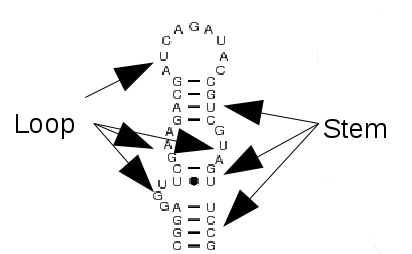
\includegraphics[width=50mm, height=35mm]{../img/struktury_v_rna-stem_loop.png}
%TODO klasicky obrazok RNA molekuly, v ktorej farbami odlisim stem a loop.
\caption{Stem a loop v molekule}
\label{obr:RNA_motifs_stem_loop}
\end{figure}








